\documentclass[12pt]{article}
\usepackage{setspace}
\usepackage{amsmath,amssymb}
\usepackage{amsfonts}
\usepackage{graphicx}
\usepackage{float}
\usepackage{pdfpages}
\usepackage{url}
\renewcommand{\UrlFont}{\small\tt}
\usepackage[utf8]{inputenc}
\usepackage[colorlinks=black,citecolor=black,urlcolor=black,bookmarks=trur,hypertexnames=true]{hyperref} 
\hypersetup{
    colorlinks=true,
    linkcolor=black,
    filecolor=magenta,      
    urlcolor=black,
}
\usepackage[round]{natbib}
\bibliographystyle{ieeetr}
\begin{document}

\hfill \\
Fundação Getúlio Vargas, Rio de Janeiro \\
Artigo para avaliação na disciplica \textbf{Modelagem de Fenômenos Biológicos} \\
\textbf{Graduandos:} Victor Vilanova e Alexandre Garriga \hfill

\smallskip\hrule\bigskip

\begin{center} \textbf{\LARGE Modelagem da COVID 19 - Portugal} \end{center}
\begin{center} 07 de dezembro de 2020 \end{center}
{\Large \textbf{Resumo}}
\newline
A COVID-19 em Portugal tem se agravado substancialmente nos últimos tempos \cite{calamidade}. Nesse sentido, forçando até o governo portugues a decretar estado de calamidade pública como último recurso a tentar apaziquar a situação da pandemia no país. Nesse sentido, realizar uma modelagem da pandemia torna-se crucial para identificar possíveis problemas e ajudar o governo a tomar medidas públicas mais efetivas contra a doença.
\newline
Nesse sentido, esse artigo apresenta um modelo SEAIR modificado, com base em um referencial teórico de artigos do Pedro Teles da Faculdade de Ciências da Universidade de Porto. Após isso, apresentaremos a metodologia utilizada, faremos cálculo do $R_0$, do nosso modelo, análise de sensibilidade, otimização dos parâmetros e uma análise bayesiana dos parâmetros propostos.
\newline
Diante disso, concluiremos a população de Portugal pode ter subestimado a gravidade da pandemia e que a grave situação atual em que o país se encontra pode estar prestes a se amenizar.

\tableofcontents
\thispagestyle{empty}


{\large \section{Introdução} }
Muito informação já se sabe sobre a Sars-CoV-2, mas conhecida como a COVID-19, uma doença transmitira por vírus altamente infectuosa. Na maioria dos casos, a infecção pelo vírus Sars-Cov-2 pode levar ao infectado contrair síndrome de dificuldade respiratória aguda (ARDS) causando insuficiência respiratória, choque séptico, falha múltipla de orgãos e até a morte. Estudos, do começo da aparição da doença na China, sugerem que a taxa de mortalidade esteja em torno de $3.5\%$. Entretanto, esse valor parece ser mais alto quando olhamos para o histórico da doença na Itália, por exemplo.
\newline
\newline
Nesse sentido, ao abordarmos a situação da efermidade em Portugal, nosso país de estudo desse artigo, a taxa de crescimento da epidemia no país foi uma das maiores da Europa. Por meados de 2 de março de 2020, havia sido observado que a taxa de crescimento de novos casos por dia da infecção foi de $34\pm13\%$, o que preocupou as autoridades. As cidades mais afetadas até o momento eram Lisboa e Porto, porém logo a doença se espalhou por todo o país.
Nesse contexto, com Portugal com um crescimento quase que exponencial da epidemia, diversas medidas de contençao tiveram que ser adotadas pelo governo, como a quarentena de pessoas nas suas casas, o fechamento de escolas \cite{fechamento_escolas}, distânciamento social e adoção de medidas de proteção antiséptica e uso de máscara obrigatório, com obejtivo de conseguir o achatamento da curva, e assim, prorrogar o pico da epidemia, desafogando hospitais e garantindo leito para os enfermos. 
\newline
\newline
Assim, com as medidas para a contenção do surto, que foi uma das mais rápidas da Europa, o país teve o pico observado dia 10 de abril de 2020, com $1516$ novos casos observados pela população, gerando declaração de estado de emergência pela alta taxa de mortes no país \cite{altasmortes} e, portanto, mais restrições de circulação para a população.
Após isso, as medidas adotadas tiveram um grande efeito sobre a epidemia local, de 1516 casos confirmados no começo de abril, cairam para 92 casos confirmados dia 03 de maio de 2020, evidênciando os efeitos positivos gerados pelas medidas de contenção.
Todavia, ao abordarmos o momento atual, dia 28 de setembro de 2020, a situação não é favorável. No começo de setembro, a taxa de novos casos diária voltou a subir no país e no dia 26 de setembro o país, que antes, estava com a epidemia de certo modo controlada, ultrapassou a barreira de 24 mil casos simultâneos, oque chamou atenção tanto das autoridades quanto da população, para não relaxamento das medidas de contenção e sua importância.
\newline \newline
Nesse contexto, a situação geral atual da epidemia de Portugal é o enfrentamento da chamada "segunda onda". A segunda onda, embora possa ser evitada ao máximo, é prevista em muitos casos de pandêmia pela incerteza de saber se aquela doença já atingiu o seu limiar, que no caso de modelos SIR adaptados é o famoso $R_0 < 1$, apenas quando esse limiar é atingído é que é seguro o relaxamento das medidas de contenção, evitando a segunda onda da doença.

{\large \section{Referencial teórico (Modelagem Matemática)} }
\newline
\subsection{Predicting the evolution of SARS-Covid-2 in Portugal using an adapter Sir Model previously used in South Korea for the MERS outbreak \cite{ref01}}
Autor: Pedro Teles 
\newline
Data: 13 de Abril de 2020\newline
Faculdade de Ciências da Univerdidade do Porto \\
\newline
Nesse artigo, Pedro Teles faz uma rica introdução sobre o início da disseminação do corona virus mundialmente e justifica usar o mesmo modelo usado para descrever MERS na Corea do Sul, pois ambas as doenças são provocadas por um vírus da familia coronavirus, e tem sintomas similares, embora a MERS tem uma taxa de mortalidade bem maior.
\newline
Nesse sentido, Pedro Teles na sua metodologia utiliza um modelo adaptado do SIR, em que S número de sucetíveis; E, número de expostos; A, número de assintomáticos; I número total de infectados; H número de casos hospitalizados; R, número de casos removidos e N, número total da população.

\begin{figure}[!h]
    \centering
    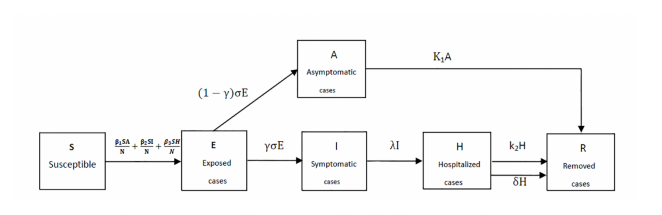
\includegraphics[scale=0.65]{trab 01.PNG}
\end{figure}
\newline

Após isso, há a declaração de parâmetros usados e, como a epidemia em Portugal não estava, de fato estabelecida ainda, ou seja, não havia dados suficientes. Pedro Teles para achar seus parâmetros usou dados da epidemia da Itália, por ser uma país vizinho e similar, como forma de estimar os devidos parâmetros.
\newline
Assim, há uma declaração de 4 possíveis cenários para Portugal, que se diferenciam de acordo com o nível de medidas, de proteção e contençao, adotadas pelo governo e população. Sendo assim, ficando explítito a recomendação da tomada de medidas de contenção.
\subsection{A time-dependent SEIR model to analyse the evolution of the Sars-CoV-2 Epidemic outbreak in Portugal \cite{ref02}}
Autor: Pedro Teles \newline
Data: 4 de Maio de 2020 \newline
Faculdade de Ciências da Univerdade do Porto
\newline
Nesse artigo, Pedro Teles, mesmo autor do artigo citado em 2.1, realiza outra modelagem de forma a mitigar os parâmetros e se adequar aos dados, agora, de Portugal. Nesse sentido, em sua introdução o autor justifica o uso de paramêtros dependentes do tempo, pois ele permite ajustar os parâmetros de acordo com o tempo que passa e, assim, as condições da epidemia que mudam ao decorrer do tempo.
\newline
\newline
Sendo assim, Pedro Teles utiliza um modelo de SEIR, em que um de seus parâmetros é dependente do tempo. Dessa vez, já se possui dados de Portugal e, se usa que 13\% dos casos de COVID-19 são hospitalizados, dado que foi retirado da análise a partir da pandemia portuguesa.
\newline \newline
Nesse sentido, o modelo é composto por S, casos sucetíveis; E, expostos; A, assintomáticos; I, infectados; H, número de casos hospitalizados; R, numero de casos removidos e N, número total da população portuguesa. Ademais, nesse modelo o parâmetro dependente do tempo é $\beta(t)$, que representa o coeficiente de transmissão dos assintomáticos, sintomáticos e casos hospitalizados para sucetíveis.
\begin{figure}[!h]
    \centering
    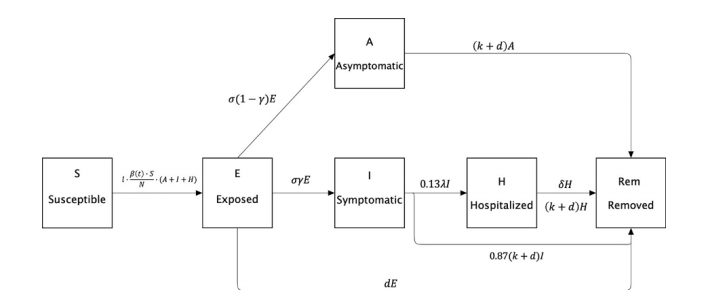
\includegraphics[scale=0.65]{trab 02.png}
\end{figure}
\newline
\newpage
Após isso, Pedro Teles acha seus parâmetros, a partir, de dados já de Portugal de modo a máximizar a semelhança com a curva de dados original.
\newline
\newline
Assim, para concluir, Pedro demonstra que pequenas mudanças nos parâmetros observados possuem grande influência na forma das curvas e, assim, na trajetória da pandemia. Desse modo, a importância de um modelo baseado no tempo para os parâmetros. E conclui, que a forma mais eficaz de controlar a disseminação da pandemia é são o uso de prevenção de proteções pessoais e medidas de isolamento.
\subsection{Predicting the evolution and control of the COVID-19
pandemic in Portugal \cite{ref03}}
Autores: Icardo J. Pais e Nuno Taveira \newline
Data: Primeira publicação: 23 de Abril de 2020; Segunda publicação: 9 de setembro de 2020 \newline
Centro de investigação Interdisciplinar Egas Moniz (CiiEM), Instituto Universitário Egas Moniz, Caparica, 2829-511, Portugal
2
\newline Research Institute for Medicines (iMed.ULisboa), Faculty of Pharmacy, University of Lisbon, Lisbon, 1649-003, Portugal
\newline
\newline
Nesse artigo, que tivemos como objeto de estudo, já se passou por uma atualização pelo fato da possibilidade de utilizar os dados captados de Portugal, e assim, melhorar o modelo e obter melhores insights que ajudaram a entender melhor a evolução do COVID-19 em Portugal. Com isso, previnir novos surtos na pandemia local.
\newline \newline
Sendo assim, os autores desse trabalho, focaram em uma abordagem simplista da pandemia e da realidade. Para isso, utilizam o modelo SI para a modelagem matemática da pandemia. Em que: S, utiliza-se para sucetíveis e I, para infectados. Segue as equações de EDO's utilizadas no modelo:
\[ \frac{dI}{dt} = k(1-\alpha) SI + \alpha k \beta S I - \frac{1}{\gamma} I \]
\[ \frac{dS}{dt} = -k(1-\alpha) SI - \alpha k \beta S I \]
Com o ajustamento dos parâmetros do modelo com os dados da pandemia obtidos de Portugal, pode-se chegar a conclusão que do início da Pandemia, entre os dias 11 e 20 de março, no país, a população em geral não implementou de fato as medidas de proteção e distânciamento impostas pelo governo, estima-se que apenas dentre 30\% a 40\% da população ficou de fato em quarentena nesse ínicio. Entretanto, após a pandemia se alastrar pelo país, estima-se que, pelo dia 19 de Agosto, dentre 70\% a 75\% da população estava respeitando todas as medidas pedidas pelo governo e da direção-geral de saúde de Portugal. Dessa maneira, mostrando uma concientização da população frente ao problema da pandemia.

{\large \section{Metodologia} }
Como Metodologia do nosso modelo epidemiológico, iremos adotar um modelo SEIAR dependente do tempo. Ou seja, nosso modelo adotado será um SEIAR em que haverá parâmetros descritos a seguir que devem variar com o tempo.
\newline
A escolha desse modelo é justificada por dois grandes motivos:
\begin{itemize}
    \item queremos modelar a epidemia de um longo período de tempo, nesse sentido, queremos buscar adequação tanto para o ínicio da pandemia em Portugal, quanto para os momentos atuais, que não são favoráveis e que indicam um novo pico epidêmico em breve.
    \item É um modelo relativamente simples de EDO's, mas que podemos retirar bastantes informações e, assim, poder gerar conclusões concretas a respeito da COVID-19 em Portugal e, até mesmo, realizar previsões a respeito do futuro da pandemia portuguesa.
\end{itemize}
\subsection{SEIAR (dependente do tempo)}
Visualização do modelo: \newline
\begin{figure}[!h]
    \centering
    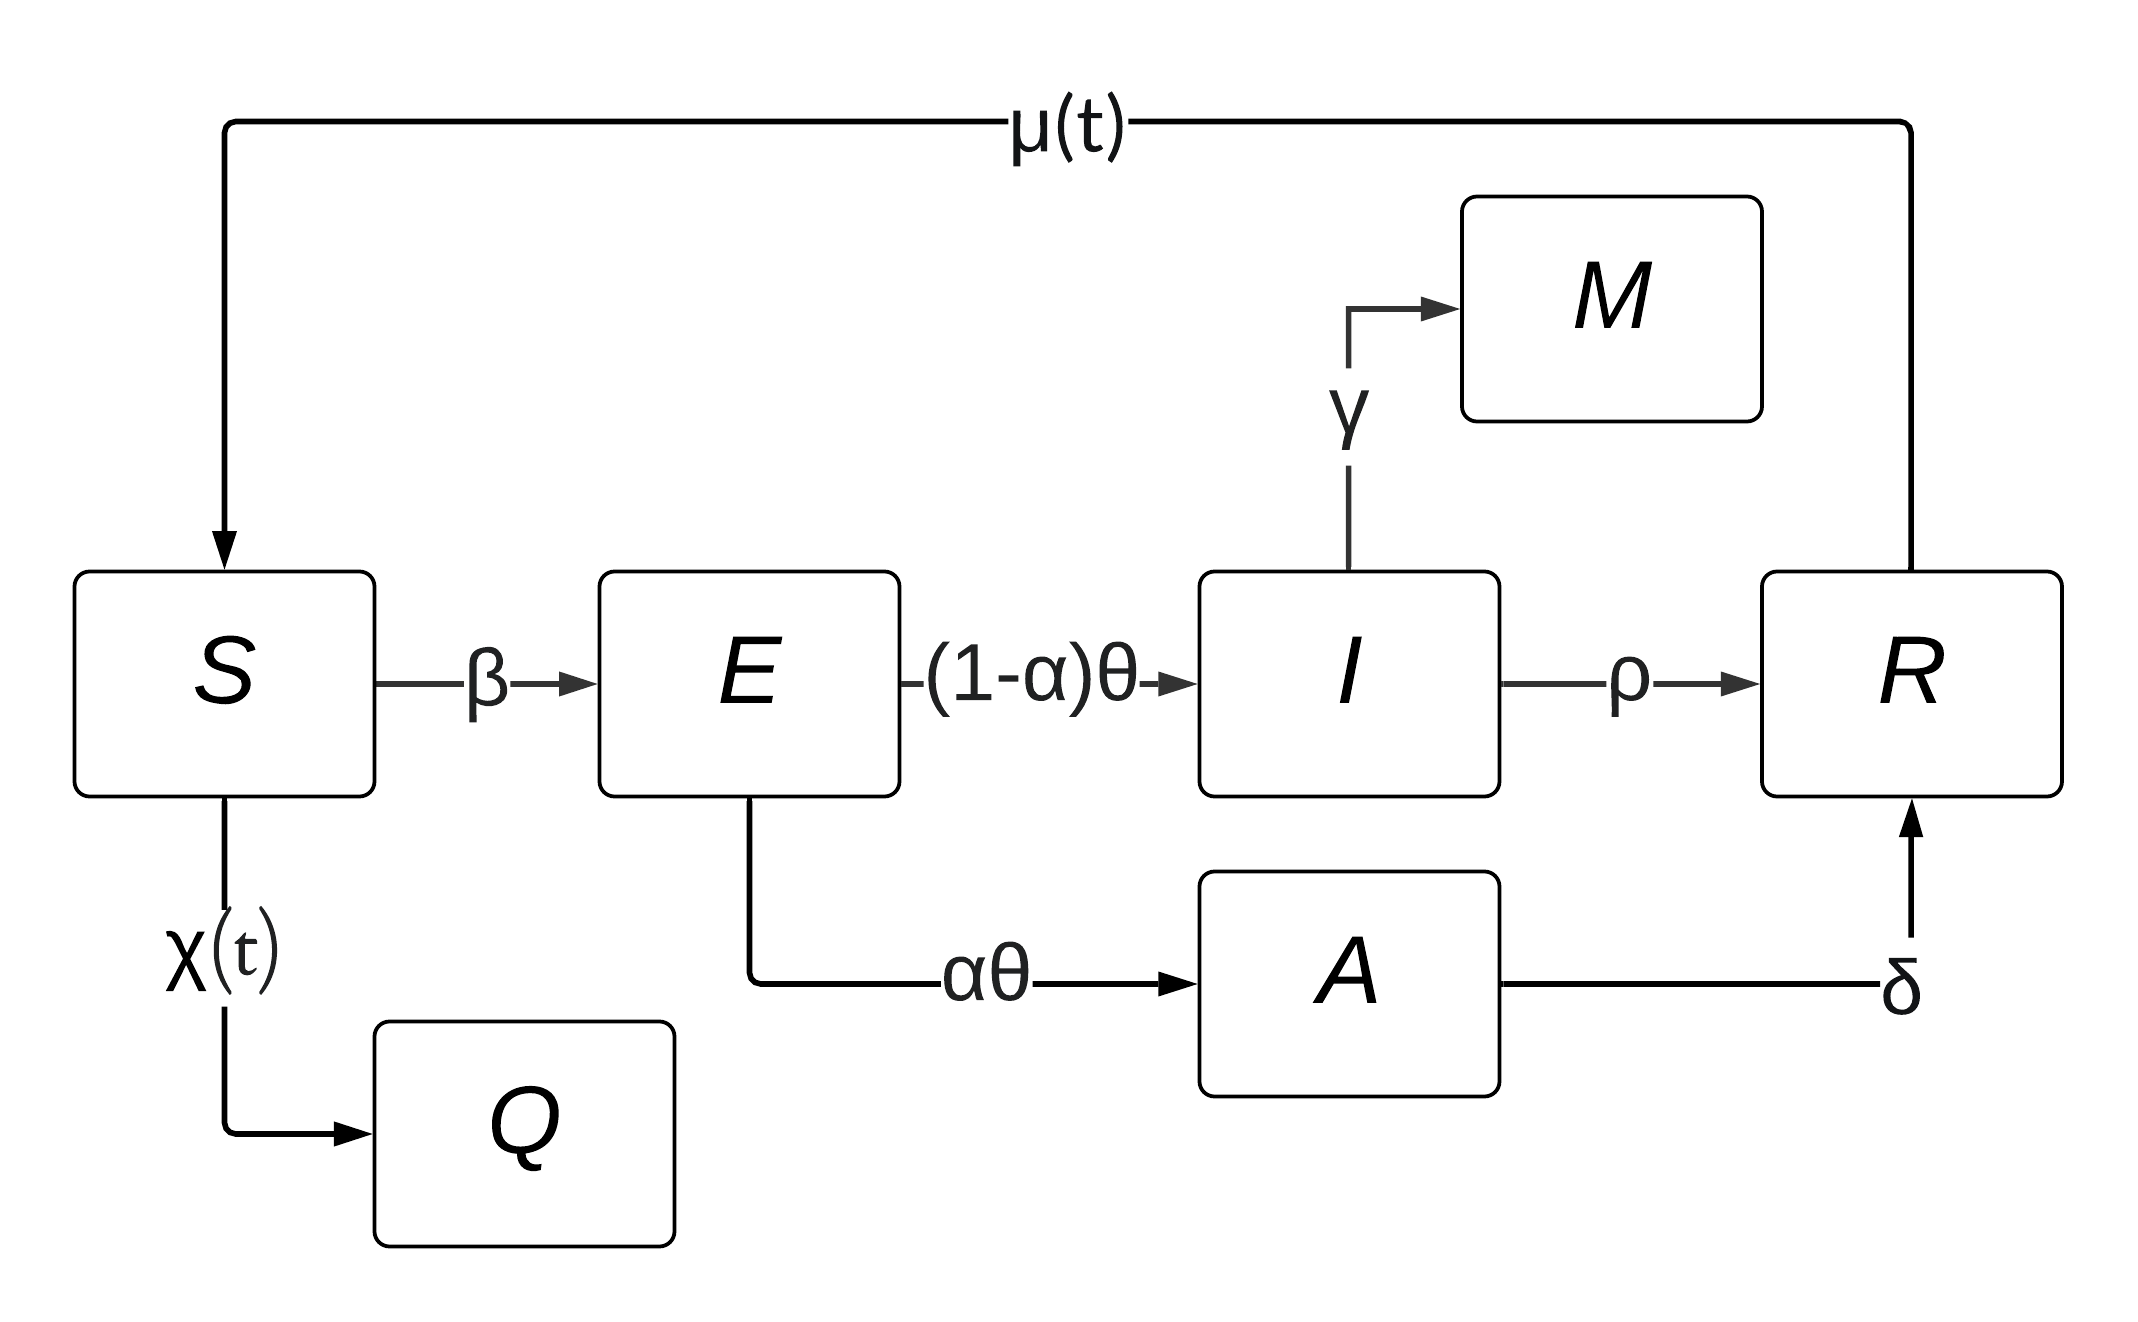
\includegraphics[scale=0.5]{reinfeccao e assintomaticos.png}
    \caption{Modelo SEIAR - dependente do tempo, feito com Lucidchart}
\end{figure}
\newline
Sendo assim, o modelo escolhido para objeto de estudo da modelagem é composto por S, Sucetíveis; E, Expostos; I, Infectados; A, Assistomáticos; M, Mortos; R, Recuperados e C, Infectados Acumulados. Observe que iremos supor que é possível a reinfecção pelo vírus, ou seja, os casos recuperados voltam a ser sucetíveis. Resolvemos isso, pois de acordo com uma pesquisa realizada pelo departamento de Microbiologia de HKU em Hong Kong \cite{reinfeccao}, observaram que é possível a reinfecção pelo vírus podendo ser um novo genoma da COVID-19.
\newline
\newline
Dos parâmetros, teremos $\beta(t)$ que será o coeficiente da taxa da população que será exposta ao vírus; $\chi(t)$ que será a taxa da população em quarentena, em função do tempo; $\alpha$ que será o coeficiente da porcentagem da população assintomática; $\beta$ será um coefinciente de normalização; $\gamma$ a taxa dos infectados que vêem a falecer; $\rho$ a taxa dos infectados que se recupera; $\delta$ a taxa dos assintomáticos que se recupera e $\mu$ a taxa dso recuperados que voltam a ser sucetíveis.
\newline
\newline
Dessa maneira, com as variáveis e parâmetros definidos, podemos montar nossas EDO's (equações diferenciais ordinárias):

\begin{align*}
  \frac{dS}{dt} &= -\beta(t)(1-\chi)SI + \mu R   \\
 \frac{dE}{dt} &= \beta(t)(1-\chi)SI - \theta E    \\
 \frac{dI}{dt} &= (1-\alpha)\theta E - \rho I - \gamma I   \\
 \frac{dA}{dt} &= \alpha \theta E - \delta A \\
 \frac{dM}{dt} &= \gamma I \\
 \frac{dR}{dt} &= \rho I + \delta A - \mu R \\
 \frac{dC}{dt} &= (1-\alpha) \theta E \\
 S + Q + E + I + A + M + R & = N
\end{align*}
\subsubsection{Análise Dimensional}

Para validarmos nosso modelo, precisamos da análise dimensional. Sendo assim, devido a natureza da taxa de variação, nossas ODE's terão unidades $[P]/[T]$ em que $[P]$ são pessoas e $[T]$ o tempo. Dessa maneira, substituindo nossas variáveis conhecidas pelas suas dimensões consequimos encontrar a dimensão dos nossos parâmetros:

\newline
De $\frac{dS}{dt}$, podemos retirar que: 
\[ \frac{[P]}{[T]} = [P] \mu \]
\[ [\mu] =\frac{1}{[T]} \] 
\[ \frac{[[P]}{[T]} = \beta[P][P] \]
\[ [\beta] = \frac{1}{[P][T]} \]
De $\frac{dE}{dt}$, podemos retirar que:
\[ \frac{[[P]}{[T]} = \theta[P] \]
\[ [\theta] = \frac{1}{[T]} \]
De $\frac{dI}{dt}$, podemos retirar que:
\[ \frac{[[P]}{[T]} = \delta[P] \]
\[ [\delta] = \frac{1}{[T]} \]
De $\frac{dA}{dt}$, podemos retirar que:
\[ \frac{[[P]}{[T]} = \gamma[P] \]
\[ [\gamma] = \frac{1}{[T]} \]
De $\frac{dM}{dt}$, podemos retirar que:
\[ \frac{[[P]}{[T]} = \rho[P] \]
\[ [\rho] = \frac{1}{[T]} \]

\subsection{Captura dos dados}

A captura dos nossos dados de interesse será feita pela própria Direção-Geral de saúde de Portugal, que disponibiliza de forma clara, eficiênte e transparente os dados e informações a respeito da COVID-19 no país.

{\large \section{Resultados} }
\subsection{Equilíbrio livre de doença}

 Do equilíbrio livre de doença do modelo, o sistema tende a permanecer no estado de equilíbrio e, para esta análise podemos desacoplar os recuperados e mortos, pois esses compartimentos não influenciam na nossa dinâmica. Assim, obtemos:
 \[ [S=r_1, E=0, I=0, A=0,R=0] \]
 
\subsection{Cálculo do R0}

Do cálculo do $R_0$, podemos entendê-lo como o número de casos secundários causados por um único caso primário. O $R_0$ do nosso modelo é:
\[ R_0 = -\frac{(\alpha-1)\beta\chi-(\alpha-1)\beta}{\rho} \]

\subsection{Simulações}

Ao gerar as curvas com nosso modelo, com base nos parâmetros que condizem com a realidade da COVID 19 mundial, $\rho$ e $\mu$ irão variar discretamente no tempo. Isso se da, a partir de uma rápida análise dos dados onde é possível ver duas etapas da pandemia de Portugal.

\begin{table}[h]
\centering
\caption{Parâmetros de teste}
\vspace{0.5cm}
\begin{tabular}{r|lr}

Parâmetro & Valor\\ % Note a separação de col. e a quebra de linhas
\hline                               % para uma linha horizontal
$\rho $ & 0.06      \\
$\beta $ & 1.42  \\
$\gamma$ & 0.03           \\
$\chi(0 \leq t \leq 50)$ & 0.40      \\
$\chi(150 \leq t \leq 200)$ & 0.2      \\
$\chi(t > 200)$ & 0.1      \\
$\alpha$ & 1.13 \\
$ \theta $ & 0.88 \\
$ \delta$ & 1.54 \\
$\mu(0 \leq t \leq 50)$ & 0.2     \\
$\mu(150 \leq t \leq 200)$ & 0.5       \\
$\mu(t > 200)$ & 0.8      \\
\end{tabular}
\end{table}
\begin{figure}[H]
    \centering
    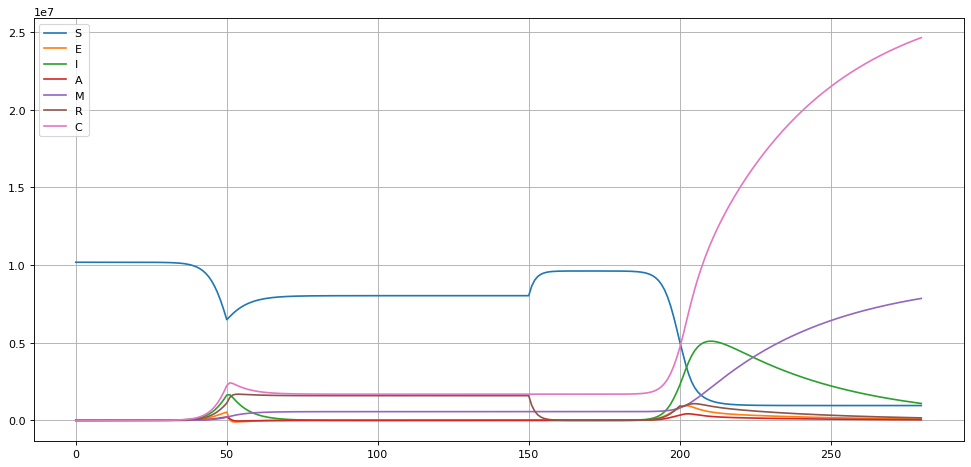
\includegraphics[scale=0.4]{simu.png}
    \caption{Simulação inicial}
\end{figure}

Diante disso, perceba que ao variar $chi$ , temos a representação da porcentagem da população que está de quarentena e ao variar $\mu$ temos a representação da chegada de um novo genoma do vírus, ou até mesmo, a reeinfecção. Ademais, veja que o modelo se encaixa na pandemia presente em Portugal.

\subsection{Análise de sensibilidade}

A análise de sensibilidade pode ser um instrumento útil para determinar a importância de uma variável sobre o resultado final de outra. Em resumo, ao variar uma variável de um determinado item, ela mostra o efeito dessa mudança no valor total. 

\begin{figure}[H]
    \centering
    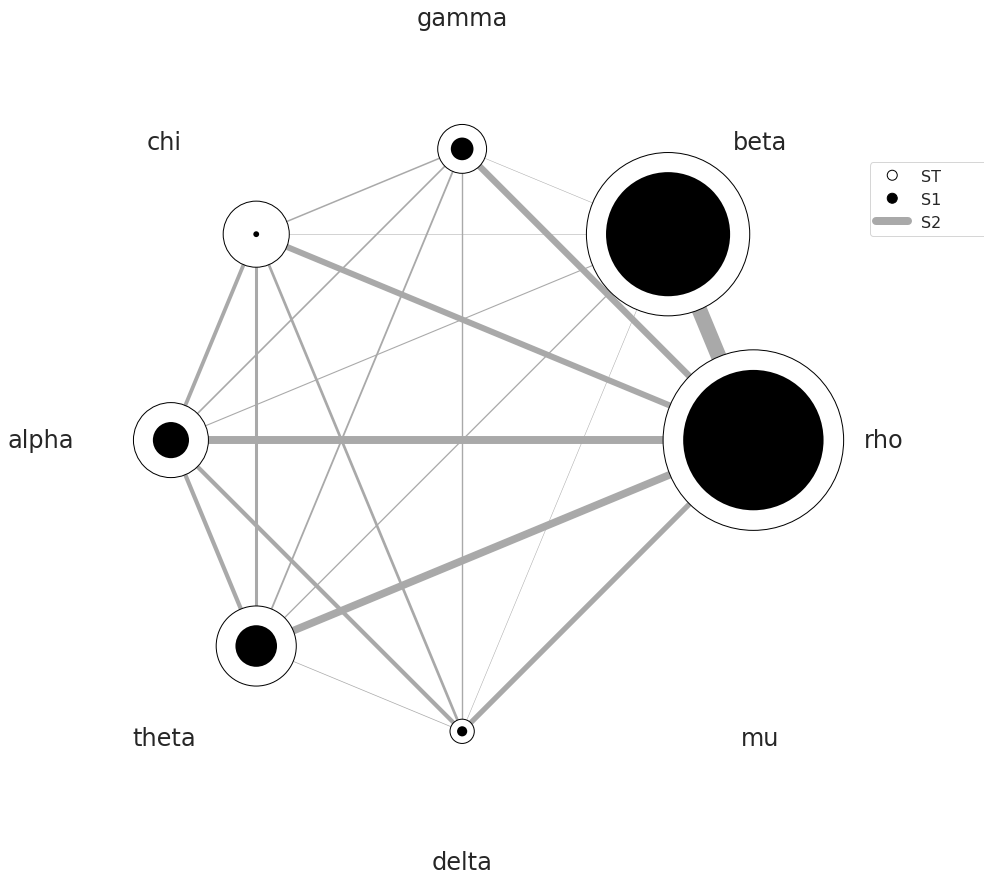
\includegraphics[scale=0.25]{sensi2.png}
    \caption{Visualização da análise de Sensibilidade}
\end{figure}
No nosso trabalho em questão, após a análise, nós podemos ver que as variáveis que mais afetam o valor total são rho e beta, ou seja, uma mudança nessas variáveis gera uma variação no valor total maior do que em comparação a outras (theta, delta, mu, gama). Uma observação importante a se fazer é que a avaliação do impacto de certas variações percentuais de uma variável sobre os indicadores de desempenho do projeto não reflete, necessariamente, a probabilidade de ocorrência dessa variação. No entanto, são dados bastantes interessantes para o nosso projeto que conseguimos obter usando esta análise.

\subsection{Otimização dos parâmetros}

A otimização dos parâmetros visa modelar o comportamento das variáveis resposta em função do ajuste dos parâmetros do processo e determinar o ajuste ótimo dos parâmetros que otimiza simultaneamente as nossas variáveis é de suma importância para a veracidade e eficácia desse nosso projeto. Sob esse viés, opós rodar otimizar os parâmetros, utilizando para isso, a biblioteca Sherpa, a fim de adequar o modelo aos dados reais vistos na pandêmia de Portugal, obtemos:
\begin{table}[h]
\centering
\caption{Parâmetros Otimizados}
\vspace{0.5cm}
\begin{tabular}{r|lr}

Parâmetro & Valor\\ % Note a separação de col. e a quebra de linhas
\hline                               % para uma linha horizontal
$\rho $ & 0.06836569577432164      \\
$\beta $ & 1.6397582054982562  \\
$\gamma$ & 0.034301858098379955           \\
$\chi(0 \leq t \leq 50)$ & 0.40      \\
$\chi(150 \leq t \leq 200)$ & 0.2      \\
$\chi(t > 200)$ & 0.1      \\
$\alpha$ & 0.496258596298859 \\
$ \theta $ & 1.2168432179798558 \\
$ \delta$ & 0.5071558607152366\\
$\mu(0 \leq t \leq 50)$ & 0.2     \\
$\mu(150 \leq t \leq 200)$ & 0.5       \\
$\mu(t > 200)$ & 0.8      \\
\end{tabular}
\end{table}

\begin{figure}[!h]
    \centering
    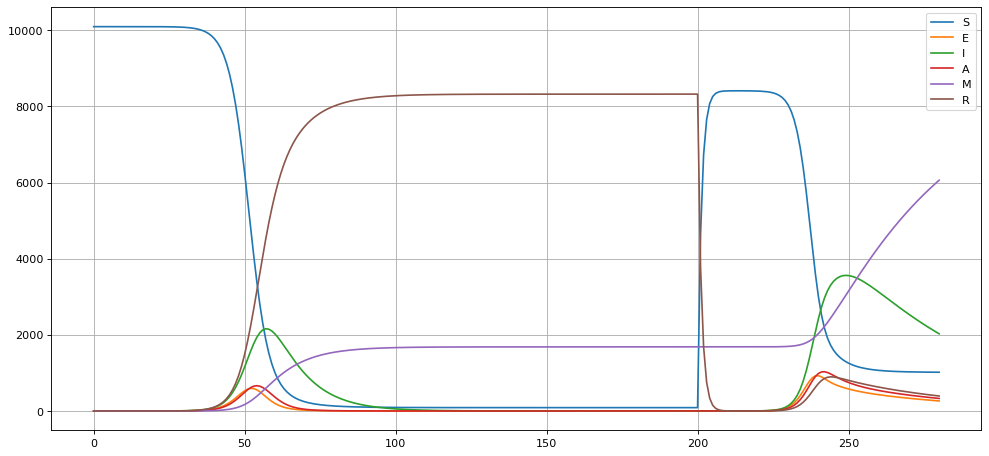
\includegraphics[scale=0.45]{plot_apos.png}
    \caption{Visualização do modelo otimizado}
\end{figure}

\newpage
\subsection{Estimação Bayesiana dos parâmetros}

O principal objetivo da inferência Bayesiana é calcular os valores esperados de funções pré definidas de um dado parâmetro. A informação a priori, a respeito da interpretação dos parâmetros, pode ser expressa utilizando-se prioris informativas ou prioris não-informativas, caso não haja opinião sólida sobre os parâmetros do modelo.
\begin{figure}[!h]
    \centering
    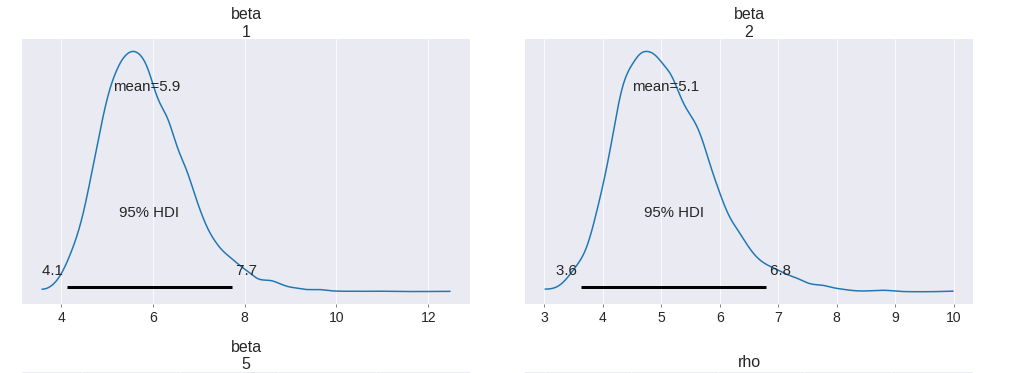
\includegraphics[scale=0.4]{baye_cortado.png}
    \caption{Resultado das distribuições a Priori dos parâmetros}
\end{figure}
{\large \section{Discussão} }

Após as análises feitas, podemos concluir que nosso modelo tem forte aplicabilidade para a adequação e entendimento da população quanto a gravidade de uma pandemia mundial dessa grandeza. Nesse sentido, é possível, com o modelo proposto, entender o comportamento da população e o desenrolar da pandemia na região de Portugal.
Fica claro, portanto, que a partir das etapas das pesquisas científicas presentes nesse artigo a covid em Portugal está sendo bem modelada e conduzida com dados bastante convincentes da direção geral de Portugal.


{\large \section{Conclusão} }

Conforme visto no nosso modelo, foi possível afirmar com precisão as diferentes porcentagens da população que ficou em quarentena. Sendo assim, foi indicada um relaxamento dos portugueses quando a primeira onda atingiu o país por volta de abril de 2020, com isso, vemos que a segunda onda, que começou por volta de setembro de 2020, foi e está bem maior que a primeira onda da doença, apresentando recordes que praticamente quadruplicaram o número máximo de casos diários em comparação ao da primeira onda.
\newline
\newline
Ademais, nosso modelo pode confirmar que o estado atual, não é bem favorável para os portugueses, porém, esse estado pode estar perto de atingir um limiar; pois nosso modelo revela que o pico do momento atual está prestes a ocorrer.
Apesar da relevância dos resultados obtidos, não podemos focar apenas em números, é necessário considerar a heterogeneidade dos indicadores entre diferentes regiões com transmissão, pois elas variam de várias formas dependendo das cidades analisadas, disponibilidade de suprimentos, questões culturais e políticas. Todos esses fatores observados são bem complexos de serem modelados de forma matemática por serem bastante abstratos e, certamente, afetam o desenrolar da pandemia em Portugal.
\newline

Sendo assim, nossa recomendação final ao governo de Portugal é que continue no decreto de calamidade pública por tempo indeterminado e continue com as restrições impostas a população a fim de desacelerar o crescimento da segunda onda de forma mais rápida possível. 
\newline

Por fim, devemos salientar que conforme novas fontes de informações e dados sobre a pandemia forem sendo revelados nosso modelo deve ser atualizado a fim de encaixar e retratar ainda melhor a realidade.

{\large \section{Referências Bibliográficas}}
\bibliography{ref.bib}


\end{document}

